\section{Detector Transfer}
\label{app:transfer}

We evaluate the $9\times9$ transfer of the frozen 36D/$K{=}28$ SIEVE Detector, with target-specific clean Mapping, across the nine model--dataset tasks. For each source $\rightarrow$ target cell, the Detector and its maximum-F1 threshold are trained and frozen on the source's Training/Validation; the target trains its Mapping only on its own fault-free executions and generates 36D Test-set features. Target Training/Validation fault labels play no role in Detector training, threshold calibration, or tuning, and target Test-set labels are used only for offline scoring. All tasks use the same random dual-bit injections, with telemetry recorded for up to 50 decoding steps. The all-finite subset requires all 36 features of target Test-set executions to be finite, serving only as a conditional diagnostic without changing predictions, models, or thresholds.

\begin{figure}[!ht]
\centering
    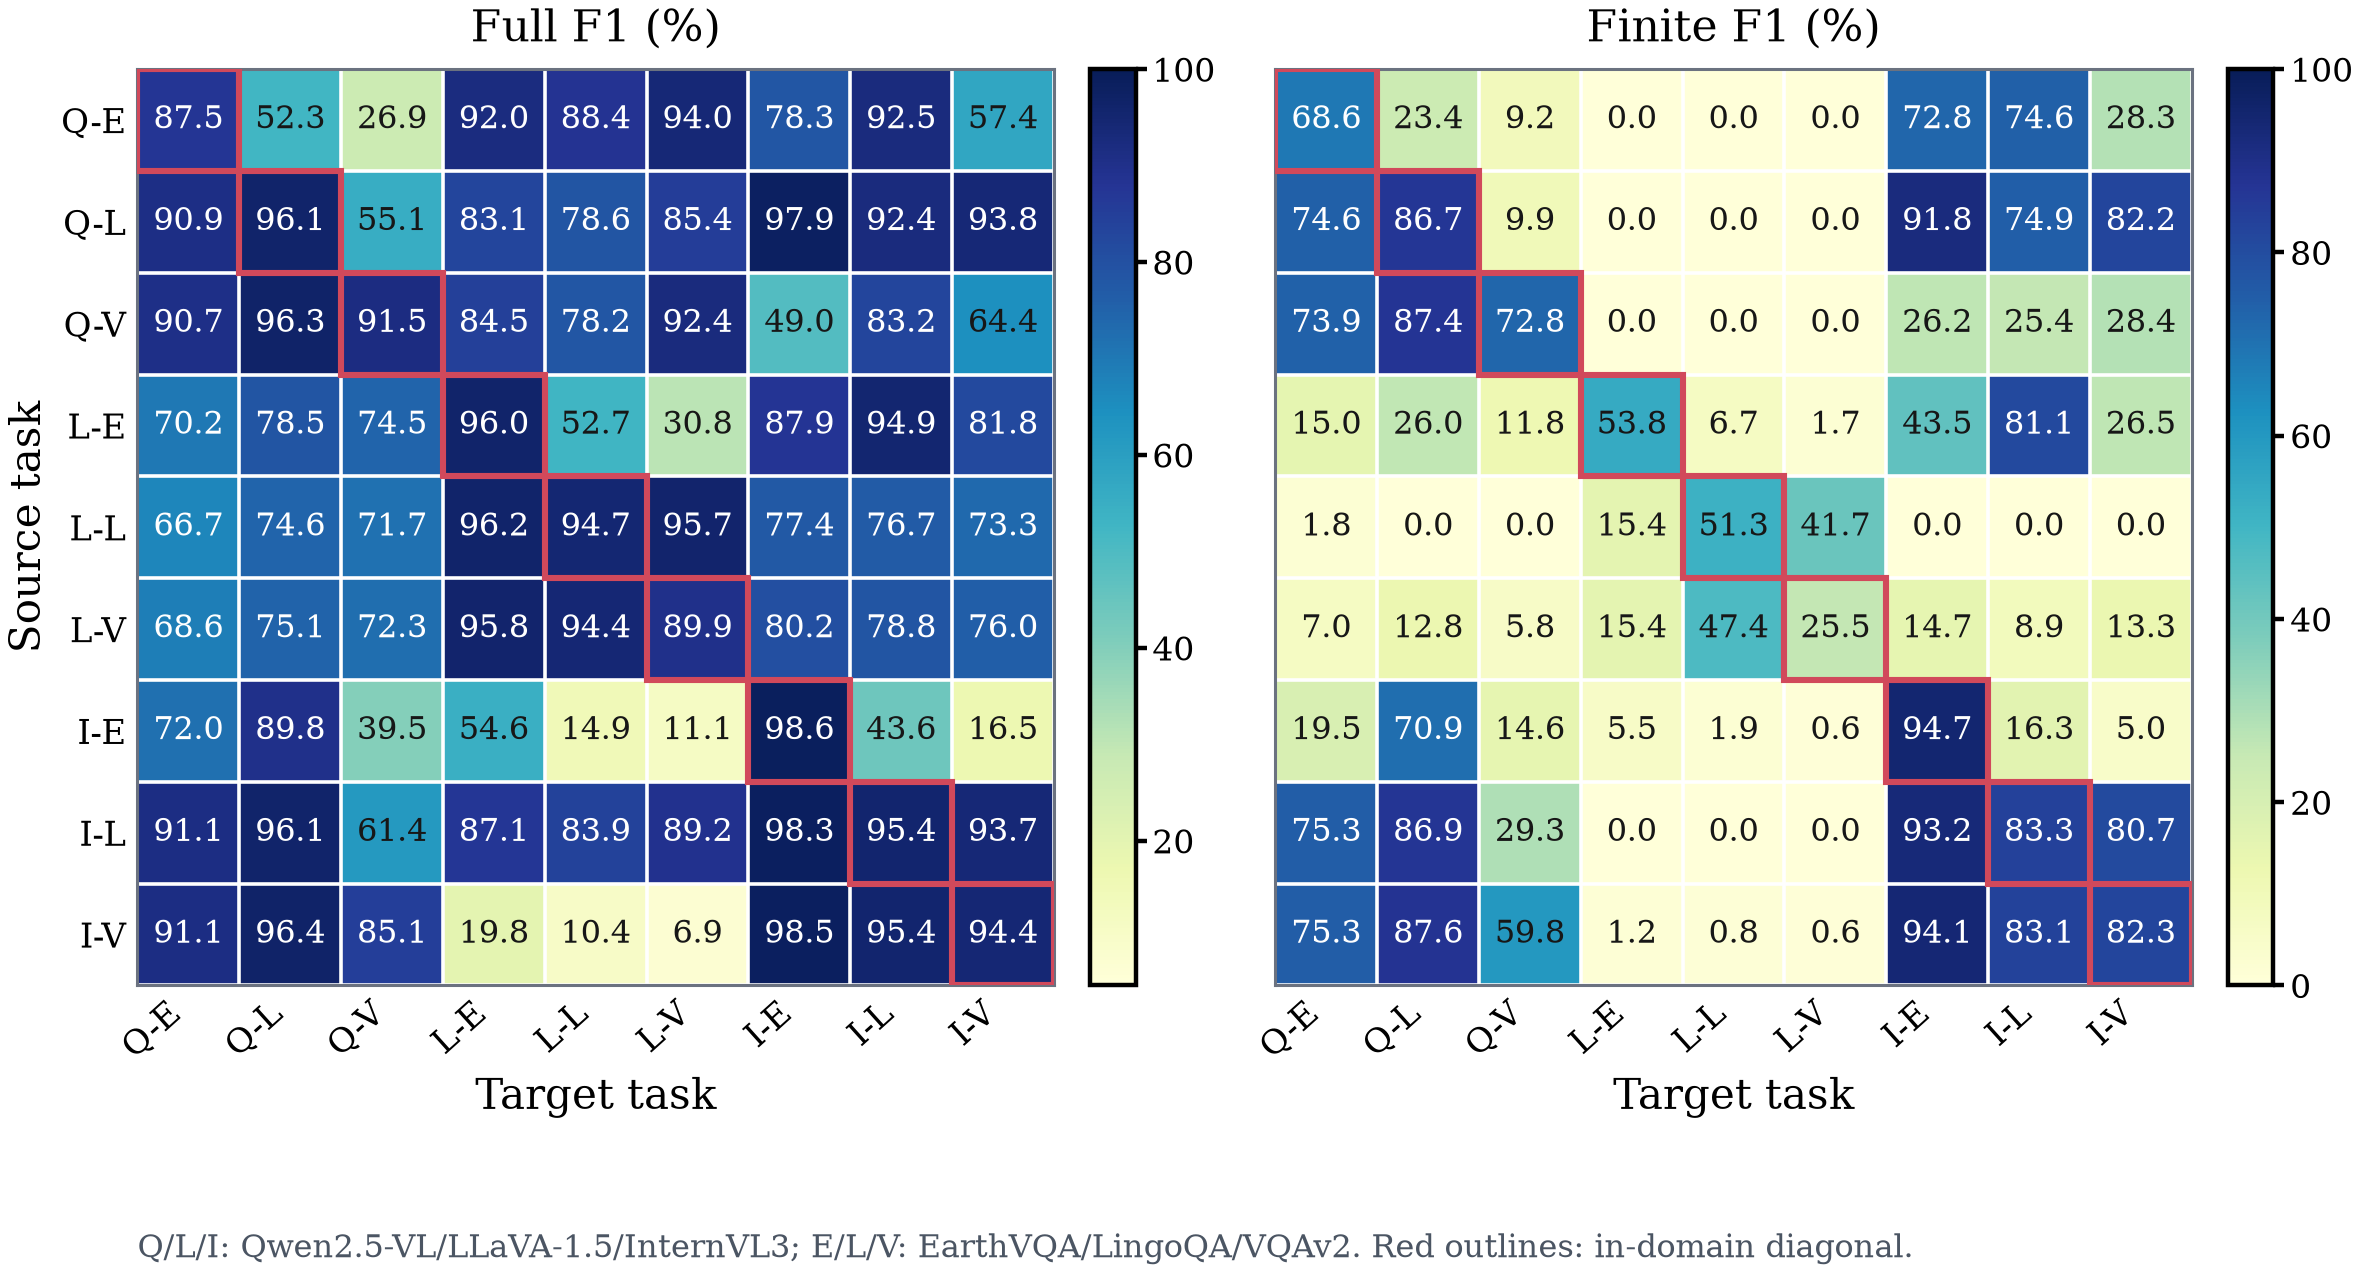
\includegraphics[width=1.0\linewidth]{Figures/figure10_transfer_F1_matrix.png}
    \caption{$9\times9$ transfer F1 (\%) of the frozen 36D/$K{=}28$ Detector. Rows are sources, columns are targets; source Detectors and thresholds are fixed, and each target uses only its own clean Mapping to generate features. Left: all retained executions; right: all-finite conditional diagnostic after configuration freezing. Red boxes mark the in-domain diagonal. Q/L/I denote Qwen2.5-VL, LLaVA-1.5, InternVL3; E/L/V denote EarthVQA, LingoQA, VQAv2.}
    \label{fig:transfer}
\end{figure}

The nine diagonal cells in Figure~\ref{fig:transfer} (all retained executions) reproduce the \S4.2.1 Test-set results item by item (macro F1 $=$ 93.78\%). Across the 72 off-diagonal cells, the macro F1 is 73.46\% with an FPR of 3.97\%, clearly higher than the 0.11\% in-domain; the macro F1 on the all-finite subset is 28.91\%, a supplementary diagnostic under fixed conditions. These results indicate that some source--target combinations transfer, but a target-specific clean Mapping remains necessary, and there is a substantial calibration mismatch between the frozen source threshold and the target distribution; this does not constitute evidence of zero-shot deployment without target-side data.

\begin{table}[!ht]
\caption{Macro-averaged Significant-SDC metrics (\%) by transfer relationship, all retained executions.}
\label{tab:A9}
\centering
\small
\begin{tabular}{lccccc}
\toprule
\textbf{Relationship} & \textbf{Cells} & \textbf{Precision} & \textbf{Recall} & \textbf{F1} & \textbf{FPR} \\
\midrule
In-domain & 9 & 96.38 & 91.49 & 93.78 & 0.11 \\
Same model, cross dataset & 18 & 71.95 & 89.14 & 73.55 & 5.81 \\
Cross model, same dataset & 18 & 90.06 & 72.64 & 75.24 & 3.19 \\
Cross model, cross dataset & 36 & 84.07 & 75.66 & 72.53 & 3.45 \\
\midrule
\textbf{Off-diagonal macro} & \textbf{72} & \textbf{82.54} & \textbf{78.28} & \textbf{73.46} & \textbf{3.97} \\
\bottomrule
\end{tabular}
\end{table}

\begin{table}[!ht]
\caption{Macro-averaged Significant-SDC metrics (\%) by transfer relationship, all-finite subset.}
\label{tab:A10}
\centering
\small
\begin{tabular}{lccccc}
\toprule
\textbf{Relationship} & \textbf{Cells} & \textbf{Precision} & \textbf{Recall} & \textbf{F1} & \textbf{FPR} \\
\midrule
In-domain & 9 & 79.88 & 62.81 & 68.78 & 0.11 \\
Same model, cross dataset & 18 & 62.09 & 54.09 & 43.28 & 5.81 \\
Cross model, same dataset & 18 & 49.68 & 25.53 & 23.67 & 3.19 \\
Cross model, cross dataset & 36 & 48.16 & 29.52 & 24.35 & 3.45 \\
\midrule
\textbf{Off-diagonal macro} & \textbf{72} & \textbf{52.02} & \textbf{34.66} & \textbf{28.91} & \textbf{3.97} \\
\bottomrule
\end{tabular}
\end{table}

Each matrix cell is bootstrapped 10{,}000 times over the target's image/question groups; per-cell F1 and 95\% CIs are provided with the accompanying reproduction results. Because the same source threshold is applied directly to different target distributions, the off-diagonal FPR and performance gaps reflect the actual transfer calibration mismatch rather than a re-selected operating point.

